\documentclass[a4paper,10.5pt,
			   bindingoffset=0.2in,left=3.35cm,right=2.12cm,top=3.75cm,bottom=2.88cm,%
				footskip=.25in
				listof=numbered,toc=chapterentrywithdots]{scrreport}

% Package Imports
\usepackage[utf8]{inputenc} % UTF-8 encoding
\usepackage[T1]{fontenc}    % Proper font encoding
\usepackage{lmodern}        % Modern font
\usepackage{graphicx}       % Graphics support
\usepackage[hidelinks]{hyperref}       % Clickable links
\usepackage{amsmath, amssymb} % Math symbols
\usepackage{listings}       % Code listings
\usepackage{csquotes}       % Quotation support
\usepackage{booktabs}       % Better tables
\usepackage{caption}        % Better captions
\usepackage{float}			% better positioning
\usepackage{tabularx}

%\documentclass[listof=numbered]{scrreprt} % making lists caputred

\usepackage[toc]{glossaries} % Glossary
\makeglossaries
\newglossaryentry{fitzpatrick-skin-type}{
	name={Fitzpatrick skin type},
	plural={Fitzpatrick skin types},
	description={A skin classifier based on the skins' reaction to ultraviolet light, developed by dermatologist Dr. Thomas Fitzpatrick \autocite{Gottfrois2024}}
}
\newglossaryentry{JupyterNotebook}{
	name={Jupyter Notebook},
	description={Executable files, often used in ML to write Python code and add explanations in text form}
}
\newglossaryentry{gpuhub}{
	name={GPUhub},
	description={\gls{HSLU}’s server infrastructure for GPU-related computing. It provides isolated environments with JupyterLab access for developing and running \gls{ML} workflows}
}
\newglossaryentry{pediatric}{
	name={pediatric},
	description={A medical term for infants, children and adolescents \autocite{Farlex_nodate}}
}
\newglossaryentry{proxyVar}{
	name={proxy variable},
	plural={proxy variables},
	description={"one or more variables that encode the protected attribute with a substantial degree of accuracy" \autocite{Wang_2021}}
}
\newglossaryentry{teledermatology}{
	name={teledermatology},
	description={dermatological care from a distance, supported by modern technology \autocite{Pala_2020}}
}
\newglossaryentry{Fairlearn}{
	name=Fairlearn,
	description={A Python library for assessing and improving fairness in machine learning models. It supports various fairness metrics and mitigation techniques, especially for binary classification tasks \autocite{Fairlearn_nodate}}
}
\newglossaryentry{Equalized-Odds-Difference}{
	name={equalized odds difference},
	description={The absolute difference in true positive and false positive rates between subgroups, used as a group fairness metric \autocite{Fairlearn_nodate}}
}
\newglossaryentry{Equalized-Odds-Ratio}{
	name={equalized odds ratio},
	description={The ratio of true positive and false positive rates between subgroups, used as a group fairness metric \autocite{Fairlearn_nodate}}
}
\renewcommand{\glossarysection}[2][]{}


\usepackage[style=apa,backend=biber]{biblatex}       % Bibliography
\addbibresource{references.bib} % Bibliography file

\usepackage{todonotes}
\usepackage{xcolor}
\renewcommand{\todo}[1]{\textcolor{red}{TODO: #1}}
%\usepackage{titlesec} for report
\renewcommand{\chapterformat}{\thechapter\autodot\enskip}


% Change chapter format in the document (no "Chapter", just number + title)
%\titleformat{\chapter}[hang]{\normalfont\huge\bfseries}{\thechapter}{1em}{}

% Ensure chapters still appear correctly in the Table of Contents
\renewcommand{\chaptermark}[1]{\markboth{\thechapter\ #1}{}}
\renewcommand{\thechapter}{\arabic{chapter}}
\renewcommand{\thesection}{\thechapter.\arabic{section}}


%\usepackage[titles]{tocloft}

% adapt toc
%\usepackage[nottoc]{tocbibind}
\usepackage{tocbasic} % Instead of tocbibind
%%\KOMAoptions{toc=chapterentrywithdots} % Ensures correct TOC formatting
%%\KOMAoptions{listof=leveldown} 

\setcounter{tocdepth}{2}


% Title Page
\title{Demographic Biases in Dermatology Models}
\author{Nadja Stadelmann}
\date{\today}

\begin{document}
	\pagenumbering{gobble}
	% Title Page
	\maketitle
	
	
	\fontsize{12}{14}
	\noindent\textbf{Bachelor Thesis at Lucerne University of Applied Sciences and Arts
		School of Computer Science and Information Technology} \\ \vspace*{0.6cm}
	
	\fontsize{10.5}{12}
	\noindent
	\textbf{Title of Bachelor Thesis:} Demographic Biases in Dermatology Models\\ \vspace*{0.2cm}
	
	\noindent
	\textbf{Name of Student:} Nadja Stadelmann\newline \newline
	\textbf{Degree Program:} BSc Computer Science \newline \newline
	\textbf{Year of Graduation:} 2025\newline \newline
	\textbf{Main Advisor:} Ludovic Amruthalingam\newline \newline
	\textbf{External Expert:} \newline \newline
	\textbf{Industry partner/provider:} Applied AI Research Lab, Lucerne University of Applied Sciences and Arts\newline \newline \newline
	\textbf{Code / Thesis Classification:}\\
	$\boxtimes$ Public (Standard) \newline
	$\square$ Private
	
	
	\todo{fix linebreaks and indents}
	\paragraph{\textbf{Declaration}}
	I hereby declare that I have completed this thesis alone and without any unauthorized or external help. I further declare that all the sources, references, literature and any other associated resources have been correctly and appropriately cited and referenced. The confidentiality of the project provider (industry partner) as well as the intellectual property rights of the Lucerne University of Applied Sciences and Arts have been fully and entirely respected in completion of this thesis. \newline \newline
	Place / Date, Signature	\underline{\hspace*{8cm}} \newline \newline
	
	\paragraph{\textbf{Submission of the Thesis to the Portfolio Database:}}
	
	Confirmation by the student \newline
	I hereby confirm that this bachelor thesis has been correctly uploaded to the Portfolio Database in line with the code of practice of the University. I rescind all responsibility and authorization after upload so that no changes or amendments to the document may be undertaken.  \newline \newline
	Place / Date, Signature	\underline{\hspace*{8cm}} \newline
	
	\newpage
	\paragraph{\textbf{Expression of thanks and gratitude}}
	
	\todo{add thanks and gratitude}
	
	Ludovic Amruthalingam
	
	Simone Lionetti - deputy Ludovic
	
	Pascal Baumann - LaTeX
	
	\newpage
	\pagenumbering{arabic}
	% Abstract
	\begin{abstract}
		\todo{Your abstract here.}
	\end{abstract}
	
	% Table of Contents
	\tableofcontents
	\listoftodos
	
	\todo{use the template on overleaf: https://www.overleaf.com/project/67cac1b71993d0b44b6ba7ee}
	\todo{Alle Fakten (fundiertes Wissen Dritter) sind korrekt zitiert. Es werden verschiedene Zitierweisen verwendet und teilweise mehrere Interpretationen gegenübergestellt. Der gemeinsam definierte Zitierstil im Text, in Abbildungen und Tabellen sowie im Literaturverzeichnis wird korrekt und durchgängig angewendet. Eigene Leistungen (sowie Bewertungen) und Fremdquellen sowie Recherchen sind klar unterscheidbar.} \linebreak
	\todo{Die erstellten Artefakte sind von sehr hoher Qualität. Das trifft u.a. auf Diagramme, Skizzen sowie Notationen (z.B. BPMN/UML) zu. Darstellungen sind einwandfrei, alle statistisch notwendigen Qualitätskriterien sind erfüllt. Beschriftungen etc. sind vorhanden, keine Einwände, Text und Bild stimmen beschreibend gut überein. Es wurden angemessene Dokumentationsmethoden und -arten korrekt verwendet. Vereinbarte Interview Transkripte, Beobachtungsprotokolle bzw. Zusammen-fassungen sind vorhanden. Daten, Ort, Kontext, Beschreibung, Zeilennummer, Verweise, Strukturen sind erkennbar, gut formatiert und korrekt mit dem Text/ der Analyse verknüpft. Alle Elemente und Themen sind im methodischen Teil/Text erklärt und verständlich, keine technischen oder strukturellen Einwände. Auch Zwischenanalysen, Zwischenschritte oder Gesamtauswertungen wurden durchgeführt, die Herkunft der Daten ist erkennbar und professionell aufbereitet.} \linebreak
	\todo{Der Schreibstil aller Dokumente entspricht hohen Standards und enthält keine Übertreibungen oder unbegründete Beurteilungen. Die Sprache ist aussagekräftig, prägnant und präzise. Die Fachterminologie ist konsistent, d.h. für gleiche Gegenstände und Themen werden immer die gleichen Begriffe verwendet. Der Sprachgebrauch ist durchgängig geschlechtergerecht, einheitlich und sachlich.}
	\todo{Portfolio DB für Referenzarbeiten anschauen}
	
	
	% Chapters
	\chapter{Problem Statement}
		\todo{Welche Ziele, Fragestellungen werden mit dem Projekt verfolgt? Die Bedeutung, Auswirkung und Relevanz dieses Projektes für die unterschiedlichen Beteiligten soll aufgeführt werden. Typischerweise wird hier ein Verweis auf die Aufgabenstellung im Anhang gemacht.}
	
		\todo{Formulate statement from those citations}:
		\begin{itemize}
			\item AI systems can be used in many sensitive environments to make important and life-changing decisions; thus, it is crucial to ensure that these decisions do not reflect discriminatory behavior toward certain groups or populations \autocite{Mehrabi_2021}.
			\item There are clear benefits to algorithmic decision-making; unlike people, machines do not become tired or bored [45, 119], and can take into account orders of magnitude more factors than people can. However, like people, algorithms are vulnerable to biases that render their decisions “unfair” [6, 121]. In the context of decision-making, fairness is \textit{the absence of any prejudice or favoritism toward an individual or group based on their inherent or acquired characteristics}. Thus, an unfair algorithm is one whose decisions are skewed toward a particular group of people. \autocite{Mehrabi_2021}.
			\item it is important for researchers and engineers to be concerned about the downstream applications and their potential harmful effects when modeling an algorithm or a system \autocite{Mehrabi_2021}.
			\item We should think responsibly, and recognize that the application of these tools, and their subsequent decisions affect peoples’ lives; therefore, considering fairness constraints is a crucial task while designing and engineering these types of sensitive tools \autocite{Mehrabi_2021}.
			\item \autocite{Mehrabi_2021}.
			\item \autocite{Mehrabi_2021}.
			
		\end{itemize}
	
		\section{Context}
			This thesis is part of the PASSION project. The PASSION research team identified that in Africa, dermatology treatment is not accessible. There is less than one dermatologist per one million citizens. In contrast, there is high demand for dermatology treatment, especially among children and adolescents. 80\% of the \gls{pediatric} population is affected. The goal of PASSION is to make dermatology treatment more accessible by using AI supported telemedicine for triage \autocite{Gottfrois2024}.
		
			For AI supported triage, demographic biases in existing dermatology models is a problem since the corresponding datasets lack diversity, especially regarding skin tones \autocite{Gottfrois2024}. This type of bias is important in dermatology, since different diseases present themselves differently depending on the skin-color \autocite{Diaz2022}. Further, skin diseases are more advanced or severe at diagnosis in patients with lower socioeconomic status \autocite{BAD2021}.
			
			PASSION tries to mitigate the demographic bias by providing a dataset of pigmented skin images of patients from Sub-Saharan Africa. The PASSION team focused on gathering data with Fitzpatrick skin type (\gls{FST}) IV, V and VI. Further, the covered conditions represent up to 80\% of the conditions in the \gls{pediatric} population, the demographic group who is most affected by skin disease \autocite{Gottfrois2024}.
			
			The PASSION dataset is complementary to the existing datasets and improves the diversity in a combined dataset. Within the dataset itself, there could potentially be further demographic biases, e.g. related to age or gender.
			 
		\section{Objective}
		The goal of this research is to
		\begin{enumerate}
			\item Identify demographic biases in dermatology AI models, using established fairness metrics.
			\item Identify mitigation strategies to minimize these biases.
			\item Assess the effectiveness of the mitigation strategies.
		\end{enumerate}
		It is important to identify the existent biases first, so that the mitigation strategies can be \todo{proceed here to reason why you chose those objectives}
		
	
	\chapter{State of Research}
		\todo{Bezogen auf die eigenen Zielsetzungen und Fragestellungen soll aufgezeigt werden, wie andere dieses oder ähnliche Probleme gelöst haben. Worauf können Sie aufbauen, was müssen Sie neu angehen?	Wodurch unterscheidet sich Ihre Lösung von anderen Lösungen? Für wissenschaftlich orientierte Arbeiten sei hier explizit auf (Balzert, S. 66 ff) verwiesen.}
		\todo{Relevante, aktuelle und fundierte Fachliteratur wurde identifiziert, kritisch geprüft und verwendet. Die Begriffe der Fragestellung sind definiert und referenziert. Der gesamte Kontext ist verknüpft und eine Abgrenzung wurde vorgenommen. All dies ist in einer leicht verständlichen Struktur formuliert und überprüft.}
	
	
		\section{PASSION for Dermatology}
			The PASSION research team provides a dataset including three analysis scripts and an AI model. For this thesis, it is important to understand which labels the dataset provides, so that the applicable bias mitigation methodologies can be chosen.
			
			The provided analysis scripts show a first insight into the demographic distribution in the dataset, such as Fitzpatrick skin type and cases per country distribution. The results of those analyses reveal first biases.
			
			There are also dermatology specific analysis scripts in regards of body localization by condition or impetigo cases. Those results 
			
			\subsection{PASSION Dataset}
			The PASSION dataset contains data from patients from four African countries. It contains 4901 images of dermatology cases and the corresponding demographic and clinical information, see \autoref{tab:PASSION_labels}. There is one record per patient and one or more corresponding images. The images are linked with the record by filename, which contains the subject\_id of the row entry. Access to the dataset can be requested via \href{https://passionderm.github.io/}{https://passionderm.github.io/} \autocite{Gottfrois2024}.
			
			\begin{table}[H]
				\centering
				\begin{tabularx}{\textwidth}{>{\hsize=.27\hsize}X>{\hsize=.27\hsize\raggedright}X>{\hsize=.46\hsize}X}
					\toprule
					\textbf{Label}       & \textbf{Data Type} & \textbf{Description}       \\ \midrule
					subject\_id          & string & Participant's unique identifier        \\
					country              & string & Country of origin of the participant   \\
					age                  & integer & Age of the participant in years       \\
					sex                  & m/f/o & Gender of the participant               \\
					fitzpatrick          & integer & \gls{FST}                \\
					body\_loc            & string (list; null-able, semicolon-separated) & Specific affected body locations \\
					impetig              & 0/1  & Presence of impetigo (1=present), may occur alone or with other conditions, affects the treatment options for coexisting conditions        \\
					conditions\_PASSION  & Eczema, Scabies, Fungal, Others & Primary diagnosed skin condition \\
					\bottomrule
				\end{tabularx}
				\caption{PASSION dataset - labels and descriptions \autocite{Gottfrois2024}}
				\label{tab:PASSION_labels}
			\end{table}
			
			\subsection{PASSION Analysis Scripts}
			With the Dataset, the PASSION research team provides a \gls{JupyterNotebook} with code examples and analysis scripts. They are listed in \autoref{tab:PASSION_scripts} with a description and an indicator, how relevant the scripts are for this thesis.
			\begin{table}[H]
			\centering
			\begin{tabularx}{\textwidth}{>{\hsize=.25\hsize\raggedright}X>{\hsize=.41\hsize}X>{\hsize=.34\hsize}X}
					\toprule
					\textbf{Script Title}       & \textbf{Description} & \textbf{Relevance - Reasoning}       \\ \midrule
		  				Linking CSV Data with Image Files & 
					  	Creates mapping between the data records and images. It further counts the cases by country  &
					  	\textbf{High} - Basis for other analysis's, potentially provides dermatological info        \\
					\hline
						Extracting and Comparing Subject IDs &
						Checks the dataset complecity and accurracy in regards of linking records and images &
						\textbf{Low} - Checks loaded data for completeness, but is not providing more insight   \\
					\hline
						Regrouping Malawi and Tanzania to EAS &
						data aggregation due to dataset size and geographical proximity &
						\textbf{Low} - Might be relevant to understand the dataset and for interpreting the results of the following scripts correctly  \\
					\hline
						Conditions by Country &
						Relationship between clinical conditions and country &
						\textbf{Medium} - Currently unsure whether this information is relevant for this thesis \todo{research relevance between country vs. clinical conditions in regards of demographic bias} \\
					\hline
						Body Localizations by Conditions &
						Shows correlation between the condition and primarily affected body parts; does not use all affected body parts listed in the data \todo{check with Philippe why this was done} &
						\textbf{Low} - While the correlation can be interesting for other research, it is not relevant for demographic biases. \\
					\hline
						Impetigo Cases            &
						Counts total number of impetigo cases as well as proportion to all cases &
						\textbf{Medium} - Currently unsure whether this information is relevant for this thesis \todo{research relevance between impedigo and demographic bias} \\
					\hline
						Distribution of Fitzpatrick Skin Types &
						Counts and visualizes the skin type distribution  &
						\textbf{High} - \gls{FST} is a demographic information   \\
					\bottomrule
				\end{tabularx}
				\caption{PASSION dataset - existing analysis scripts \autocite{Gottfrois2024} \todo{decide on a table style}}
				\label{tab:PASSION_scripts}
			\end{table}	
			
			\subsection{PASSION Experiments}
			see https://github.com/Digital-Dermatology/PASSION-Evaluation
			
			
		\section{General ML biases}
			\begin{itemize}
				\item These biased predictions stem from the hidden or neglected biases in data or algorithms \autocite{Mehrabi_2021}.
				\item two potential sources of unfairness in machine learning outcomes - those that arise from biases in the data and those that arise from the algorithms ... we observe that biased algorithmic outcomes might impact user experience, thus generating a feedback loop between data, algorithms and users that can perpetuate and even amplify existing sources of bias \autocite{Mehrabi_2021}.
				\item Bias in facial recognition systems [128] and recommender systems [140] have also been largely studied and evaluated and in many cases shown to be discriminative towards certain populations and subgroups. In order to be able to address the bias issue in these applications, it is important for us to know where these biases are coming from and what we can do to prevent them.\autocite{Mehrabi_2021}.
				\item We should think responsibly, and recognize that the application of these tools, and their subsequent decisions affect peoples’ lives; therefore, considering fairness constraints is a crucial task while designing and engineering these types of sensitive tools \autocite{Mehrabi_2021}.
				\item compared SAVRY, a tool used in risk assessment frameworks that includes human intervention in its process, with automatic machine learning methods in order to see which one is more accurate and more fair. Conducting these types of studies should be done more frequently, but prior to releasing the tools in order to avoid doing harm \autocite{Mehrabi_2021}.
				\item \textbf{Assessment Tools} An interesting direction that researchers have taken is introducing tools that can assess the amount of fairness in a tool or system. For example, Aequitas [136] is a toolkit that lets users to test models with regards to several bias and fairness metrics for different population subgroups. Aequitas produces reports from the obtained data that helps data scientists, machine learning researchers, and policymakers to make conscious decisions and avoid harm and damage toward certain populations. AI Fairness 360 (AIF360) is another toolkit developed by IBM in order to help moving fairness research algorithms into an industrial setting and to create a benchmark for fairness algorithms to get evaluated and an environment for fairness researchers to share their ideas [11]. These types of toolkits can be helpful for learners, researchers, and people working in the industry to move towards developing fair machine learning application away from discriminatory behavior \autocite{Mehrabi_2021}.
			\end{itemize}	
				
			\begin{itemize}
				\item Most AI systems and algorithms are data driven and require data upon which to be trained. Thus, data is tightly coupled to the functionality of these algorithms and systems. In the cases where the underlying training data contains biases, the algorithms trained on them will learn these biases and reflect them into their predictions. As a result, existing biases in data can affect the algorithms using the data, producing biased outcomes. Algorithms can even amplify and perpetuate existing biases in the data.\autocite{Mehrabi_2021}.
				\item In addition, algorithms themselves can display biased behavior due to certain design choices, even if the data itself is not biased. The outcomes of these biased algorithms can then be fed into real-world systems and affect users’ decisions, which will result in more biased data for training future algorithms.\autocite{Mehrabi_2021}.
				\item The loop capturing this feedback between biases in data, algorithms, and user interaction is illustrated in Figure 1. We use this loop to categorize definitions of bias in the section below \autocite{Mehrabi_2021}.
				\begin{figure}[H]
					\centering
					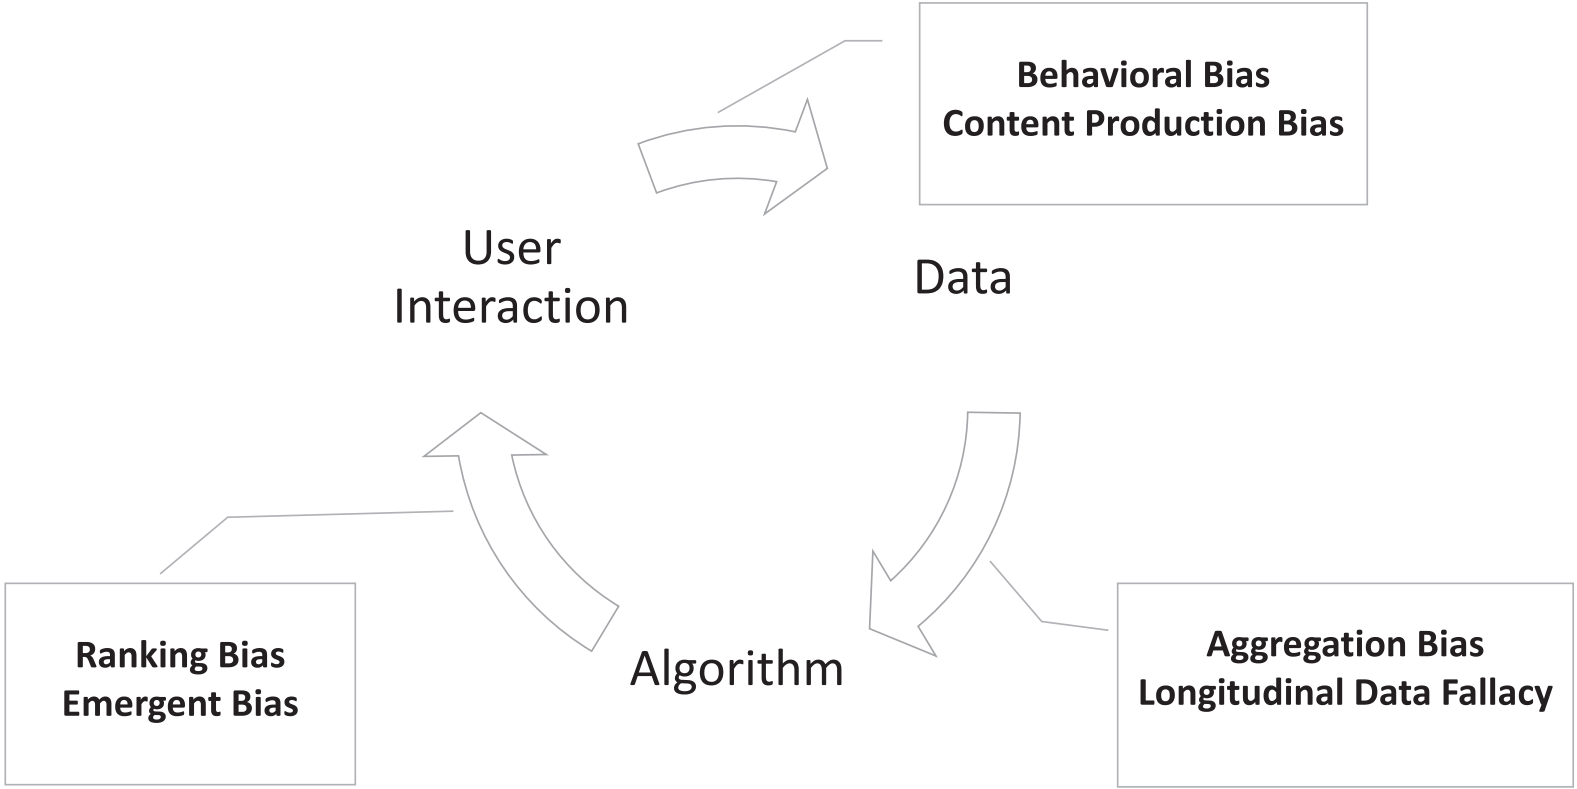
\includegraphics[width=0.8\textwidth]{figures/BiasCategoriesInMLLifecycle.png}
					\caption{Bias definitions in a ML lifecycle \autocite{Mehrabi_2021}.}
					\label{fig:example}
				\end{figure}
				\item Bias can exist in many shapes and forms, some of which can lead to unfairness in different downstream learning tasks. In [144], authors talk about sources of bias in machine learning with their categorizations and descriptions in order to motivate future solutions to each of the sources of bias introduced in the paper. In [120], the authors prepare a complete list of different types of biases with their corresponding definitions that exist in different cycles from data origins to its collection and its processing.\autocite{Mehrabi_2021}.
				\item \autocite{Mehrabi_2021}.
				\item \autocite{Mehrabi_2021}.
				\item \autocite{Mehrabi_2021}.
				\item \autocite{Mehrabi_2021}.
				\item \autocite{Mehrabi_2021}.
			\end{itemize}	
			
			Already rewritten: The following categorization was modeled with the intent to show that the different biases are intertwined and one should consider the effects between each other in the cycle to address them correctly \autocite{Mehrabi_2021}
			
			Data biases (data to algorithm (biases in data which might have an impact on biased algorithmic outcomes \autocite{Mehrabi_2021}))
			\begin{itemize}
				\item Measurement Bias. Measurement, or reporting, bias arises from how we choose, utilize, and measure particular features [144] (e.g. mismeasured proxy variables (= "one or more variables that encode the protected attribute with a substantial degree of accuracy" according to https://medium.com/bcggamma/practice-ai-responsibly-with-proxy-variable-detection-42c2156ad986)) \autocite{Mehrabi_2021}. (= e.g. someone who lives at that postal code probably has this ethnicity https://medium.com/bcggamma/practice-ai-responsibly-with-proxy-variable-detection-42c2156ad986); --> could that be an issue with the country of origin feature?
				\item Omitted Variable Bias. Omitted variable bias4 occurs when one or more important variables are left out of the model [38, 114, 131]. Something that the model was not ready for\autocite{Mehrabi_2021}. did not take into account
				\item Representation Bias. Representation bias arises from how we sample from a population during data collection process [144]. Non-representative samples lack the diversity of the population, with missing subgroups and other anomalies \autocite{Mehrabi_2021}.
				\item Aggregation Bias. Aggregation bias (or ecological fallacy) arises when false conclusions are drawn about individuals from observing the entire population. An example of this type of bias can be seen in clinical aid tools. Consider diabetes patients who have apparent morbidity differences across ethnicities and genders. Specifically, HbA1c levels, that are widely used to diagnose and monitor diabetes, differ in complex ways across genders and ethnicities. Therefore, a model that ignores individual differences will likely not be well-suited for all ethnic and gender groups in the population [144]. This is true even when they are represented equally in the training data. Any general assumptions about subgroups within the population can result in aggregation bias. \autocite{Mehrabi_2021}. --> could also be important for dermatology issues!!!
				\begin{itemize}
					\item Simpson’s Paradox. Simpson’s paradox is a type of aggregation bias that arises in the analysis of heterogeneous data [18]. The paradox arises when an association observed in aggregated data disappears or reverses when the same data is disaggregated into its underlying subgroups (Fig. 2(a)). ... After analyzing graduate school admissions data, it seemed like there was bias toward women, a smaller fraction of whom were being admitted to graduate programs compared to their male counterparts. However, when admissions data was separated and analyzed over the departments, women applicants had equality and in some cases even a small advantage over men. The paradox happened as women tended to apply to departments with lower admission rates for both genders. Simpson’s paradox has been observed in a variety of domains, including biology [37], psychology [81], astronomy [109], and computational social science [91].\autocite{Mehrabi_2021}.	
					\item Modifiable Areal Unit Problem is a statistical bias in geospatial analysis, which arises when modeling data at different levels of spatial aggregation [56]. This bias results in different trends learned when data is aggregated at different spatial scales \autocite{Mehrabi_2021}.
				\end{itemize}
				\item Sampling Bias. Sampling bias is similar to representation bias, and it arises due to nonrandom sampling of subgroups. As a consequence of sampling bias, the trends estimated for one population may not generalize to data collected from a new population. \autocite{Mehrabi_2021}. This is what the PASSION dataset tries to improve
				\item Longitudinal Data Fallacy. Researchers analyzing temporal data must use longitudinal analysis to track cohorts over time to learn their behavior. Instead, temporal data is often modeled using cross-sectional analysis, which combines diverse cohorts at a single time point. The heterogeneous cohorts can bias cross-sectional analysis, leading to different conclusions than longitudinal analysis \autocite{Mehrabi_2021}. --> could this be relevant for the progress of a specific disease? Or would that only be an issue when the progress of the disease would be predicted?
				\item Linking Bias. Linking bias arises when network attributes obtained from user connections, activities, or interactions differ and misrepresent the true behavior of the users [120] \autocite{Mehrabi_2021}. --> probably less important since we got individuals? Or could that be an issue with the country of origin feature?
				\item \autocite{Mehrabi_2021}.
				\item \autocite{Mehrabi_2021}.
				\item \autocite{Mehrabi_2021}.
			\end{itemize}	
						
			Algorithmic biases (Algorithm to user (A modulates U behaviour, biases in algorithm might lead to introduce biases in user behaviour and affect it as a consequence)) \autocite{Mehrabi_2021}
			\begin{itemize}
				\item Algorithmic Bias. Algorithmic bias is when the bias is not present in the input data and is added purely by the algorithm [9]. The algorithmic design choices, such as use of certain optimization functions, regularizations, choices in applying regression models on the data as a whole or considering subgroups, and the general use of statistically biased estimators in algorithms [44], can all contribute to biased algorithmic decisions that can bias the outcome of the algorithms.\autocite{Mehrabi_2021}.
				\item User Interaction Bias. User Interaction bias is a type of bias that can not only be observant on the Web but also get triggered from two sources—the user interface and through the user itself by imposing his/her self-selected biased behavior and interaction [9]. This type of bias can be influenced by other types and subtypes, such as presentation and ranking biases. \autocite{Mehrabi_2021}. -- more relevant for later, when the application would become bigger
				\begin{itemize}
					\item Presentation Bias. Presentation bias is a result of how information is presented [9] (can only click on content they see, could be the case that user does not see all info on web) \autocite{Mehrabi_2021}.
					\item Ranking Bias. The idea that top-ranked results are the most relevant and important will result in attraction of more clicks than others. This bias affects search engines [9] and crowdsourcing applications [93].\autocite{Mehrabi_2021}.
				\end{itemize}
				\item Popularity Bias. Items that are more popular tend to be exposed more. However, popularity metrics are subject to manipulation—for example, by fake reviews or social bots [117]. ... this presentation may not be a result of good quality; instead, it may be due to other biased factors. \autocite{Mehrabi_2021}.
				\item Emergent Bias. Emergent bias occurs as a result of use and interaction with real users. This bias arises as a result of change in population, cultural values, or societal knowledge usually some time after the completion of design [53]. This type of bias is more likely to be observed in user interfaces, ... This type of bias can itself be divided into more subtypes, as discussed in detail in [53]. \autocite{Mehrabi_2021}. probably less relevant at the first stage
				\item Evaluation Bias. Evaluation bias happens during model evaluation [144]. This includes the use of inappropriate and disproportionate benchmarks for evaluation of applications such as Adience and IJB-A benchmarks. These benchmarks are used in the evaluation of facial recognition systems that were biased toward skin color and gender [24], and can serve as examples for this type of bias [144]. \autocite{Mehrabi_2021}. -- important for this thesis
			\end{itemize}
			
			User to Data (user-generated data, inherent biases in users could be reflected in the data they generate; biases in last section might introduce further bias in this process) \autocite{Mehrabi_2021}
			\begin{itemize}
				\item Historical Bias. Historical bias is the already existing bias and socio-technical issues in the world and can seep into from the data generation process even given a perfect sampling and feature selection [144]. ... search results were of course reflecting the reality, but whether or not the search algorithms should reflect this reality is an issue worth considering \autocite{Mehrabi_2021} - maybe relevant
				\item Population Bias. Population bias arises when statistics, demographics, representatives, and user characteristics are different in the user population of the platform from the original target population [120]. Population bias creates non-representative data. ... More such examples and statistics related to social media use among young adults according to gender, race, ethnicity, and parental educational background can be found in [64]. \autocite{Mehrabi_2021}
				\item Self-Selection Bias. Self-selection bias4 is a subtype of the selection or sampling bias in which subjects of the research select themselves. \autocite{Mehrabi_2021}
				\item Social Bias. Social bias happens when others’ actions affect our judgment [9]. (case where we want to rate or review an item with a low score, but when influenced by other high ratings, we change our scoring thinking that perhaps we are being too harsh [9, 151].) \autocite{Mehrabi_2021}
				\item Behavioral Bias. Behavioral bias arises from different user behavior across platforms, contexts, or different datasets [120]. \autocite{Mehrabi_2021} maybe, people from different countries go to the dermatologist for different diseases, based on cultural differences?
				\item Temporal Bias. Temporal bias arises from differences in populations and behaviors over time [120]. \autocite{Mehrabi_2021} -- could this also be differences in the year, when people go to dermatologists? over which timeline has the PASSION data been captured? 
				\item Content Production Bias. Content Production bias arises from structural, lexical, semantic, and syntactic differences in the contents generated by users [120]. \autocite{Mehrabi_2021} -- could the quality of the pictures been related to this as well?
				\item \autocite{Mehrabi_2021}
				\item \autocite{Mehrabi_2021}
				\item \autocite{Mehrabi_2021}
				\item \autocite{Mehrabi_2021}
				\item \autocite{Mehrabi_2021}
			\end{itemize}
		
		
			Data bias examples and mitigation ideas
			\begin{itemize}
				\item Bias in ML Data - IJB-A / Adience imbalanced (mainly light-skinned subjects) - Bias towards dark-skinned groups (underrepresented). Other instance - when we do not consider different subgroups in the data. Considering only male-female groups not enough, use race to further subdivide gender groups. Only then, clear biases in sub groups can be found, since otherwise part of the groups would  compromise the other group and hide the underlaying bias towards that subgroup \autocite{Mehrabi_2021}
				\item Popular machine-learning datasets that serve as a base for most of the developed algorithms and tools can also be biased—which can be harmful to the downstream applications that are based on these datasets. ... In [142], researchers showed that these datasets suffer from representation bias and advocate for the need to incorporate geographic diversity and inclusion while creating such datasets. \autocite{Mehrabi_2021}
				\item Examples of Data Bias in Medical Applications. These data biases can be more dangerous in other sensitive applications. For example, in medical domains there are many instances in which the data studied and used are skewed toward certain populations—which can have dangerous consequences for the underrepresented communities. [98] showed how exclusion of African-Americans resulted in their misclassification in clinical studies, so they became advocates for sequencing the genomes of diverse populations in the data to prevent harm to underrepresented populations \autocite{Mehrabi_2021} \todo{What does sequencing data mean?, is it relevant}
				\item Other such studies were conducted in [54] which states that UK Biobank, a large and widely used genetic dataset, may not represent the sampling population. Researchers found evidence of a “healthy volunteer” selection bias. [150] has other examples of studies on existing biases in the data used in the medical domain. [157] also looks at machine-learning algorithms and data utilized in medical fields, and writes about how artificial intelligence in health care has not impacted all patients equally.\autocite{Mehrabi_2021}
				\item \autocite{Mehrabi_2021}
				\item \autocite{Mehrabi_2021}
			\end{itemize}
		
			Discrimination vs. bias
			\begin{itemize}
				\item bias and discrimination = source of unfairness. Discrimination can be considered as a source for unfairness that is due to human prejudice and stereotyping based on the sensitive attributes, which may happen intentionally or unintentionally, while bias can be considered as a source for unfairness that is due to the data collection, sampling, and measurement. Although bias can also be seen as a source of unfairness that is due to human prejudice and stereotyping, in the algorithmic fairness literature it is more intuitive to categorize them as such according to the existing research in these areas. In this survey, we mainly focus on concepts that are relevant to algorithmic fairness issues. \autocite{Mehrabi_2021}
				\item Explainable Discrimination. Differences in treatment and outcomes amongst different groups can be justified and explained via some attributes in some cases. In situations where these differences are justified and explained, it is not considered to be illegal discrimination and hence called explainable [77]. In [77], authors present a methodology to quantify the explainable and illegal discrimination in data. They argue that methods that do not take the explainable part of the discrimination into account may result in non-desirable outcomes, so they introduce a reverse discrimination which is equally harmful and undesirable. They explain how to quantify and measure discrimination in data or a classifier’s decisions which directly considers illegal and explainable discrimination.\autocite{Mehrabi_2021}
				\item Unexplainable Discrimination. In contrast to explainable discrimination, there is unexplainable discrimination in which the discrimination toward a group is unjustified and therefore considered illegal. Authors in [77] also present local techniques for removing only the illegal or unexplainable discrimination, allowing only for explainable differences in decisions. These are preprocessing techniques that change the training data such that it contains no unexplainable discrimination. We expect classifiers trained on this preprocessed data to not capture illegal or unexplainable discrimination. Unexplainable discrimination consists of direct and indirect discrimination.\autocite{Mehrabi_2021}
				\begin{itemize}
					\item Direct Discrimination. Direct discrimination happens when protected attributes of individuals explicitly result in non-favorable outcomes toward them [164]. ... these traits that are considered to be “protected” or “sensitive” attributes in computer science literature  \autocite{Mehrabi_2021}
					\item Indirect Discrimination. In indirect discrimination, individuals appear to be treated based on seemingly neutral and non-protected attributes; however, protected groups, or individuals still get to be treated unjustly as a result of implicit effects from their protected attributes \autocite{Mehrabi_2021}
				\end{itemize}
			\end{itemize}
			
			Algorithmic Fairness
			\begin{itemize}
				\item in order to be able to fight against discrimination and achieve fairness, one should first define fairness. \autocite{Mehrabi_2021}
				\item The fact that no universal definition of fairness exists shows the difficulty of solving this problem [138]. Different preferences and outlooks in different cultures lend a preference to different ways of looking at fairness, which makes it harder to come up with just a single definition that is acceptable to everyone in a situation. there is still no clear agreement on which constraints are the most appropriate for those problems. \autocite{Mehrabi_2021}
				\item Broadly, fairness is the absence of any prejudice or favoritism towards an individual or a group based on their intrinsic or acquired traits in the context of decision-making [139]. Even though fairness is an incredibly desirable quality in society, it can be surprisingly difficult to achieve in practice. \autocite{Mehrabi_2021}
				\item Here we will reiterate and provide some of the most widely used definitions, along with their explanations inspired from [149].\autocite{Mehrabi_2021}
				\item Definitions on page 12, 13, 14 \autocite{Mehrabi_2021}
				\begin{itemize}
					\item Equalized Odds (TP and FP rate should be the same for individuals in different sub groups) \autocite{Mehrabi_2021}
					\item Equal Opportunity (TP rate should be the same) \autocite{Mehrabi_2021}
					\item Demographic Parity / Statistical Parity (likelihood of positive outcome the same regardless of protected group) \autocite{Mehrabi_2021}
					\item Fairness Through Awareness (similar predictions to similar individuals (similarity = inverse distance)) \autocite{Mehrabi_2021}
					\item Fairness Through Unawareness (no protected attributes explicitly used in decision-making process) \autocite{Mehrabi_2021}
					\item Treatment Equality (Ration FN and FP same for both protected group categories) \autocite{Mehrabi_2021}
					\item Test Fairness (for predicted probability scores, people in both groups must have equal probability of TP) \autocite{Mehrabi_2021}
					\item Counterfactual Fairness (same outcome in actual world and counterfactual world where the individual belonged to a different demographic group) \autocite{Mehrabi_2021}
					\item Fairness in Relational Domains (“A notion of fairness that is able to capture the relational structure in a domain—not only by taking attributes of individuals into consideration but by taking into account the social, organizational, and other connections between individuals” [50]) \autocite{Mehrabi_2021} probably not relevant since not relational
					\item Conditional Statistical Parity (people in both groups have equal possibilities of being assigned to a positive outcome given a set of legitimate factors) \autocite{Mehrabi_2021}
					\item My text: The survey categorizes those fairness notions in three different groups: Individual Fairness, Group Fairness and Subgroup fairness.  \autocite{Mehrabi_2021}
					\item Subgroup fairness: Subgroup fairness intends to obtain the best properties of the group and individual notions of fairness. It is different than these notions but uses them in order to obtain better outcomes. It picks a group fairness constraint like equalizing false positive and asks whether this constraint holds over a large collection of subgroups [79][80]\autocite{Mehrabi_2021}
					\item it is impossible to satisfy some of the fairness constraints at once except in highly constrained special cases. In [83], the authors show the inherent incompatibility of two conditions: calibration and balancing the positive and negative classes. These cannot be satisfied simultaneously with each other unless under certain constraints; therefore, it is important to take the context and application in which fairness definitions need to be used into consideration and use them accordingly [141]\autocite{Mehrabi_2021}
					\item Another important aspect to consider is time and temporal analysis of the impacts that these definitions may have on individuals or groups. In [95] authors show that current fairness definitions are not always helpful and do not promote improvement for sensitive groups—and can actually be harmful when analyzed over time in some cases. They also show that measurement errors can also act in favor of these fairness definitions; therefore, they show how temporal modeling and measurement are important in evaluation of fairness criteria and introduce a new range of trade-offs and challenges toward this direction. It is also important to pay attention to the sources of bias and their types when trying to solve fairness-related questions. \autocite{Mehrabi_2021}
					\item \autocite{Mehrabi_2021}
					\item \autocite{Mehrabi_2021}
				\end{itemize}
			\end{itemize}
			
			Methods for Fair Machine Learning
			
			\begin{itemize}
				\item While this section is largely domain-specific, it can be useful to take a cross-domain view. Generally, methods that target biases in the algorithms fall under three categories \autocite{Mehrabi_2021}
				\item Pre-processing. Pre-processing techniques try to transform the data so that the underlying discrimination is removed [43]. If the algorithm is allowed to modify the training data, then pre-processing can be used [11].\autocite{Mehrabi_2021}
				\item In-processing. In-processing techniques try to modify and change state-of-the-art learning algorithms in order to remove discrimination during the model training process [43]. If it is allowed to change the learning procedure for a machine learning model, then in-processing can be used during the training of a model— either by incorporating changes into the objective function or imposing a constraint [11, 14].\autocite{Mehrabi_2021}
				\item Post-processing. Post-processing is performed after training by accessing a holdout set which was not involved during the training of the model [43]. If the algorithm can only treat the learned model as a black box without any ability to modify the training data or learning algorithm, then only post-processing can be used in which the labels assigned by the black-box model initially get reassigned based on a function during the post-processing phase [11, 14].\autocite{Mehrabi_2021}
				\item \autocite{Mehrabi_2021}
				\item \autocite{Mehrabi_2021}
			\end{itemize}
			\todo{move on with page 13-15}
		
			\subsection{ML biases}
			
			\subsection{ML fairness metrics}
			
			\subsection{ML mitigation methods}
			
	
	\chapter{Ideas and Concepts}
		\todo{Hier geht es um die Fragestellung, wie Sie die formulierten Ziele der Arbeit erreichen wollen. Sie halten z.B. erste, grobe Ideen, skizzenhafte Lösungsansätze fest. Gibt es mehrere Wege, Ansätze um dieses Ziel zu erreichen, begründen Sie hier, warum Sie einen bestimmten Weg einschlagen. Beispiel für ein Softwareprojekt: Erste Gedanken über eine grobe Systemarchitektur. Ist z.B. eine Microservice-Architektur angebracht? Welche Alternativen bestehen, wo gibt es Problempunkte? Die Umsetzung, die Beurteilung der Machbarkeit und die detaillierte Beschreibung der umgesetzten Architektur sind dann Teil der Realisierung.}
		
		\section{PASSION Dataset}
			\todo{write things to consider more precisely:}
			\begin{itemize}
				\item Include more details in gender attribute - transgender have probably different genes / hormones, and should be indicated for more accurraccy
				\item include profession / at least an adapted version to indicate high risk patients for certain diseases? -> might lead to other biases?
				\item change country of origin to ethnicity (less of a proxy variable)
				\item are the data collectors specialized in some fields? That could lead to bias towards the center's country and the diagnosed diseases
			\end{itemize}
			
		\section{Broad Methodology}
			\todo{write things to consider more precisely:}
			\begin{itemize}
				\item Divide and Conquer vs. All-In-One-Model (either by etnicity x algorithms at a time or one which seperates the imgs first by demographic subgroup (incl. Fitzpatrick skin type))
				\item BLIND performance vs. Including the demographic data
			\end{itemize}
	
	\chapter{Methods}
		\todo{Hier halten Sie fest und begründen, welches Vorgehensmodell Sie für Ihr Projekt wählen. Sie verweisen allenfalls auf die daraus entstandenen, konkreten Terminpläne mit Meilensteinen, welche z.B. unter Realisierung (Kapitel 5) oder im Anhang versorgt sind. Bei Projekten mit einer verlangten wissenschaftlichen Tiefe werden hier die geplanten Forschungsmethoden wie quantitative/qualitative Interviews, Befragungen, Beobachtungen, Feldexperiment etc. beschrieben und begründet. Warum ist in Ihrer Situation ein Interview besser als eine Umfrage? Wer soll interview werden?}
		\todo{Die gewählten Methoden sind nachvollziehbar und begründet. Eine methodische Übersicht (Methodisches BigPicture) wurde aufgezeigt und Abgrenzungen erläutert.}
	
	\chapter{Execution}
		\todo{Dies ist das Hauptkapitel Ihrer Arbeit! Hier wird die Umsetzung der eigenen Ideen und Konzepte (Kapitel 3) anhand der gewählten Methoden (Kapitel 4) beschrieben, inkl. der dabei aufgetretenen Schwierigkeiten und Einschränkungen.}
		\todo{Die gewählten Methoden werden systematisch, konsistent und korrekt auf den Kontext der Arbeit angewendet. Die Bearbeitungs- bzw. Forschungsobjekte sind einheitlich benannt, im Kontext dargestellt und sinnvoll in die Arbeit integriert. Praxis- und Erfahrungswissen (z.B. aus Interviews) wird zur Validierung und Ergänzung der erarbeiteten Ergebnisse herangezogen. }
	
	\chapter{Evaluation and Validation}
		\todo{Auswertung und Interpretation der Ergebnisse. Nachweis, dass die Ziele erreicht wurden, oder warum	welche nicht erreicht wurden.}
		\todo{Die Ziele / Forschungsfragen sind dem Umfang der Arbeit entsprechend sehr klar abgegrenzt; sie sind präzise, überprüfbar und nach den Standards der Zielformulierung definiert. Die Zielerreichung wurde systematisch und korrekt validiert.}
		\todo{Die Herleitung und Bedeutung der Ergebnisse, mögliche Varianten, Gütekriterien und eine Validierung allgemein werden nachvollziehbar diskutiert}
	
	\chapter{Outlook}
		\todo{Reflexion der eigenen Arbeit, ungelöste Probleme, weitere Ideen.}
		\todo{Die Ergebnisse und Empfehlungen schaffen einen konkreten Mehrwert für die Auftraggebenden. Einschränkungen und Grenzen werden kritisch diskutiert und die nächsten Schritte im Ausblick festgehalten, so dass die Ergebnisse direkt in der Praxis weiterverwendet und/oder angewendet werden können.}
	
	% Lists and References
	\chapter{\glossaryname}
	\printglossary[title={}]


	\todo{Add to ToC of content somehow and fix chapter numbers}
	

	\listoffigures
	
	\listoftables
	\todo{Add List of Formulas if necessary}
	\todo{add AI declarations somewhere}
	
	
	\chapter{\bibname}
	\printbibliography[heading=none]

	
	% Appendix
	\appendix
	\chapter{Appendix}
		\todo{Projektspezifisch können weitere Dokumentationsteile angefügt werden wie: Aufgabenstellung, Projektmanagement-Plan/Bericht, Testplan/Testbericht, Bedienungsanleitungen, Details zu Umfragen, detaillierte Anforderungslisten, Referenzen auf projektspezifische Daten in externen Entwicklungs- und Datenverwaltungstools etc.}
	
\end{document}
